\documentclass[UTF8,a4paper,10pt]{ctexart}
\usepackage[left=3.17cm, right=3.17cm, top=2.74cm, bottom=2.74cm]{geometry}
\usepackage{amsmath}
\usepackage{graphicx,subfig}
\usepackage{float}
\usepackage{cite}
\usepackage{caption}
\usepackage{enumerate}
\usepackage{booktabs} %表格
\usepackage{multirow}
\newcommand{\tabincell}[2]{\begin{tabular}{@{}#1@{}}#2\end{tabular}}  %表格强制换行
%-------------------------字体设置--------------
\usepackage{times} 
\setmainfont{TimesNewRomanPSMT}%英文一律使用times new roman
%楷体\kaishu  黑体\heiti 仿宋\fangsong 隶书\lishu  幼圆\youyuan
% \setCJKmainfont[BoldFont=Kaiti SC Bold]{Kaiti SC}   %大概是唯一一个有粗体的楷体_(:з」∠)_
\setCJKfamilyfont{kt}[BoldFont=Kaiti SC Bold]{Kaiti SC}
\newcommand{\kt}{\CJKfamily{kt}}  
\newcommand{\song}{\CJKfamily{song}}    % 宋体
\newcommand{\fs}{\CJKfamily{fs}}             % 仿宋体
\setCJKfamilyfont{hwkt}{STKaiti} %引用华文楷体
\newcommand{\hwkt}{\CJKfamily{hwkt}} 
\setCJKfamilyfont{hwxk}{STXingkai} %引用华文行楷
\newcommand{\hwxk}{\CJKfamily{hwxk}}
\newcommand{\yihao}{\fontsize{26pt}{36pt}\selectfont}           % 一号, 1.4 倍行距
\newcommand{\erhao}{\fontsize{22pt}{28pt}\selectfont}          % 二号, 1.25倍行距
\newcommand{\xiaoer}{\fontsize{18pt}{18pt}\selectfont}          % 小二, 单倍行距
\newcommand{\sanhao}{\fontsize{16pt}{24pt}\selectfont}  %三号字
\newcommand{\xiaosan}{\fontsize{15pt}{22pt}\selectfont}        % 小三, 1.5倍行距
\newcommand{\sihao}{\fontsize{14pt}{21pt}\selectfont}            % 四号, 1.5 倍行距
\newcommand{\banxiaosi}{\fontsize{13pt}{19.5pt}\selectfont}    % 半小四, 1.5倍行距
\newcommand{\xiaosi}{\fontsize{12pt}{18pt}\selectfont}            % 小四, 1.5倍行距
\newcommand{\dawuhao}{\fontsize{11pt}{11pt}\selectfont}       % 大五号, 单倍行距
\newcommand{\wuhao}{\fontsize{10.5pt}{15.75pt}\selectfont}    % 五号, 单倍行距
%-------------------------章节名----------------
\usepackage{ctexcap} 
\CTEXsetup[name={,、},number={ \chinese{section}}]{section}
\CTEXsetup[name={(,)},number={\chinese{subsection}}]{subsection}
\CTEXsetup[name={,.},number={\arabic{subsubsection}}]{subsubsection}
%-------------------------页眉页脚--------------
\usepackage{fancyhdr}
\pagestyle{fancy}
\lhead{\kaishu \leftmark}
% \chead{}
\rhead{\kaishu 系统综合课程设计实验报告}%加粗\bfseries 
\lfoot{}
\cfoot{\thepage}
\rfoot{}
\renewcommand{\headrulewidth}{0.1pt}  
\renewcommand{\footrulewidth}{0pt}%去掉横线
\newcommand{\HRule}{\rule{\linewidth}{0.5mm}}%标题横线
\newcommand{\HRulegrossa}{\rule{\linewidth}{1.2mm}}
%-----------------------伪代码------------------
\usepackage{algorithm}  
\usepackage{algorithmicx}  
\usepackage{algpseudocode}  
\floatname{algorithm}{Algorithm}  
\renewcommand{\algorithmicrequire}{\textbf{Input:}}  
\renewcommand{\algorithmicensure}{\textbf{Output:}} 
\usepackage{lipsum}  
\makeatletter
\newenvironment{breakablealgorithm}
  {% \begin{breakablealgorithm}
   \begin{center}
     \refstepcounter{algorithm}% New algorithm
     \hrule height.8pt depth0pt \kern2pt% \@fs@pre for \@fs@ruled
     \renewcommand{\caption}[2][\relax]{% Make a new \caption
       {\raggedright\textbf{\ALG@name~\thealgorithm} ##2\par}%
       \ifx\relax##1\relax % #1 is \relax
         \addcontentsline{loa}{algorithm}{\protect\numberline{\thealgorithm}##2}%
       \else % #1 is not \relax
         \addcontentsline{loa}{algorithm}{\protect\numberline{\thealgorithm}##1}%
       \fi
       \kern2pt\hrule\kern2pt
     }
  }{% \end{breakablealgorithm}
     \kern2pt\hrule\relax% \@fs@post for \@fs@ruled
   \end{center}
  }
\makeatother
%------------------------代码-------------------
\usepackage{xcolor} 
\usepackage{listings} 
\lstset{ 
basicstyle=\small,
escapeinside=``,
keywordstyle=\color{ blue!70} \bfseries,
commentstyle=\color{red!50!green!50!blue!50},% 
stringstyle=\ttfamily,% 
extendedchars=false,% 
linewidth=\textwidth,% 
numbers=left,% 
numberstyle=\tiny \color{blue!50},% 
frame=trbl% 
rulesepcolor= \color{ red!20!green!20!blue!20} 
}
%------------超链接----------
\usepackage[colorlinks,linkcolor=black,anchorcolor=blue]{hyperref}
%------------------------TODO-------------------
\usepackage{enumitem,amssymb}
\newlist{todolist}{itemize}{2}
\setlist[todolist]{label=$\square$}
% for check symbol 
\usepackage{pifont}
\newcommand{\cmark}{\ding{51}}%
\newcommand{\xmark}{\ding{55}}%
\newcommand{\done}{\rlap{$\square$}{\raisebox{2pt}{\large\hspace{1pt}\cmark}}\hspace{-2.5pt}}
\newcommand{\wontfix}{\rlap{$\square$}{\large\hspace{1pt}\xmark}}
%------------------------水印-------------------
\usepackage{tikz}
\usepackage{xcolor}
\usepackage{eso-pic}

\newcommand{\watermark}[3]{\AddToShipoutPictureBG{
\parbox[b][\paperheight]{\paperwidth}{
\vfill%
\centering%
\tikz[remember picture, overlay]%
  \node [rotate = #1, scale = #2] at (current page.center)%
    {\textcolor{gray!80!cyan!30!magenta!30}{#3}};
\vfill}}}
%----------------------------------------------
\begin{document}
\begin{titlepage}
    \begin{center}
    
\includegraphics[width=0.8\textwidth]{fig/NKU.png}\\[1cm]    
    \textsc{\Huge \kaishu{\textbf{南\ \ \ \ \ \ 开\ \ \ \ \ \ 大\ \ \ \ \ \ 学}} }\\[0.9cm]
    \textsc{\huge \kaishu{\textbf{计\ \ 算\ \ 机\ \ 学\ \ 院}}}\\[0.5cm]
    \textsc{\Large \textbf{系统综合课程设计实验报告}}\\[0.8cm]
    \HRule \\[0.9cm]
    { \LARGE \bfseries PA2实验报告}\\[0.4cm]
    \HRule \\[2.0cm]
    \centering
    \textsc{\LARGE \kaishu{\ \ \ \ 周辰霏1712991}}\\[0.5cm]
    \textsc{\LARGE \kaishu{年级\ :\ 2017级}}\\[0.5cm]
    \textsc{\LARGE \kaishu{专业\ :\ 计算机科学与技术}}\\[0.5cm]
    \vfill
    {\Large \today}
    \end{center}
\end{titlepage}
%----------------------------------------没想好摘要写什么不写了-----------------------------------------------------------
% \newpage
% \thispagestyle{empty}
% \renewcommand{\abstractname}{\kaishu \sihao \textbf{摘要}}
%     \begin{abstract}
%         \kt{实现基于Phong模型的光线跟踪渲染器,实现全部基础功能以及任意obj文件的渲染和纹理的附加功能。 

%         在此附上\href{https://github.com/TiffanyChou21/COSC-0035-CG/tree/master/Phong}{GitHub仓库}以及\href{https://cdn.jsdelivr.net/gh/TiffanyChou21/CDN/video/Phong.mp4}{演示Demo}  }   
%         \noindent  %顶格
%         \kt{\textbf{\\\ 关键字:}\textbf{Phong模型;光线跟踪;蒙特卡罗;C++} \\\ \\\ } 
%     \end{abstract}
%---------------------------------------------------------------------------------------------------
\tableofcontents
%---------------------------------------------------------------------------------------------------
\newpage
\watermark{60}{10}{PA2}
\setcounter{page}{1}
\section{概述}
%——————————————————————————————————————
\subsection{实验目的}
\kt{
    \begin{itemize}
        \item 学习指令周期与指令执行过程,并简单实现现代指令系统
        \item 学习运行时环境与AM的基本原理,深入理解NEMU的本质
        \item 了解基础设施测试、调试的基本框架与思想
        \item 学习IO设备的基本实现
        \item 深入理解冯诺依曼计算机体系结构并尝试在NEMU中实现
    \end{itemize}

    PA2承接PA1完成的基本部分完成x86的主要指令以运行全部的cputest实现CPU基本的指令执行功能并学习运行时环境、AM等内容继续完善调试用基础设施。最后根据已有的IO设备支持实现简单的CPU对IO设备的控制。并最终可以实现幻灯片的轮换播放以及打字游戏,同时也可在NEMU中直接运行Mario游戏。
}
%——————————————————————————————————————
\subsection{实验内容}
\kt{
    PA2实验涉及现代指令系统的实现、抽象机器AM 的原理与应用、输入输出设备三部分
    \begin{enumerate}
        \item 了解指令周期与指令执行的原理,实现几个简单指令,在NEMU中运行第一个 C 程序dummy
        \item 继续完善指令系统,学习 运行时环境和AM的基本原理,更新调试、测试的基础设施——实现DiffTest
        \item 学习IO原理,简单实现 CPU 对输入输出设备的控制
    \end{enumerate}
}
%---------------------------------------------------------------------------------------------------
\section{阶段一}
%——————————————————————————————————————
\subsection{dummy.c运行}
\kt{
    一个指令周期可以被抽象为取指→译码→执行→更新eip,虽然我们只用实现jnz、dec、inc就可以实现全部的可计算任务,但是NEMU做出来是服务于我们而不是让我们更痛苦,所以我们要实现更多有效指令来帮助我们更好的实现软件运行。

    在$/nexus-am/tests/cputest/$中执行$make\  ARCH=x86-nemu\  ALL=dummy\ run$,结合生成的$nexus-am/tests/cputest/build/dummy-x86-nemu.txt$反汇编文件以及monitor的报错信息可以得出这个什么也没有干的c文件需要我们实现call、push、sub、xor、pop以及ret指令。
    
    而在RTFSC和阅读实验指导书之后可以总结出执行流程:($/nemu/src/cpu/exec/exec.c/$中$exec\_wrapper$函数)将当前cpu的eip保存到$decoding.seq\_eip$中并将其作为参数传入$exec\_real$。在$exec\_real$中通过$instr\_fetch$取出$decoding.seq\_eip$对应的指令,查阅$opcode\_table$得到操作数对应的宽度并通过$set\_width$设置宽度,最后调用$idex$进行译码和执行,执行主要通过$make\_DHelper$这个宏实现。之后$exec\_real$函数返回到$exec\_wrapper$,再通过$update\_eip$更新eip的值,就完成了一个指令周期,周而复始就构成了一个不停计算的TRM。

    由于操作数有不同类型,根据指导书指路查看i386官方手册的Appendix\  A可以找到以下内容,以及两个NEMU独有的操作数类型代表带符号立即数的SI和寄存器al、ax、eax的a
    \begin{figure}[H]
        \centering
        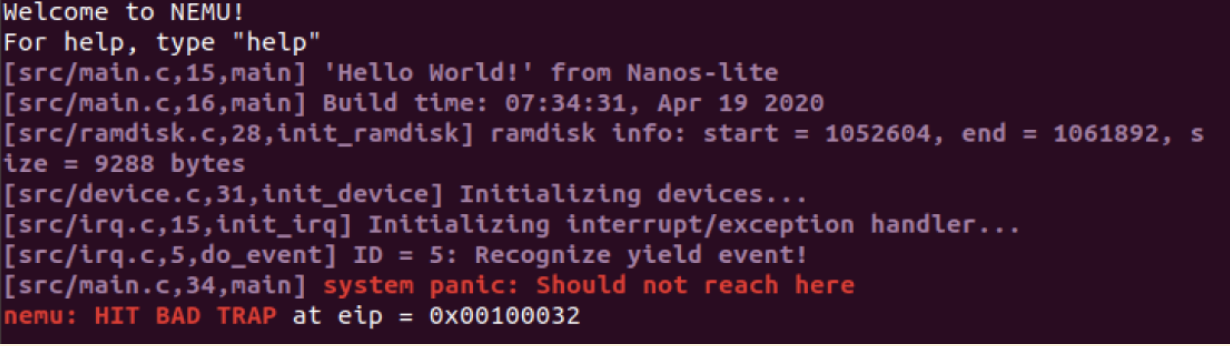
\includegraphics[scale=0.3]{fig/1.jpeg}
        \caption{Appendix \ A}
    \end{figure}

    而我们需要做的部分只有:在opcode\_table对应位置填写正确的译码函数,执行函数以及操作数宽度;在allinstr.h中声明执行函数(可省);在exec文件夹中对应文件实现执行函数,必要时借助rtl.h中声明过的RTL(可省)

    根据报错内容在i386手册中找到以下指令内容
    \begin{figure}[!h]
        \begin{minipage}[h]{0.5\linewidth}
        \centering
        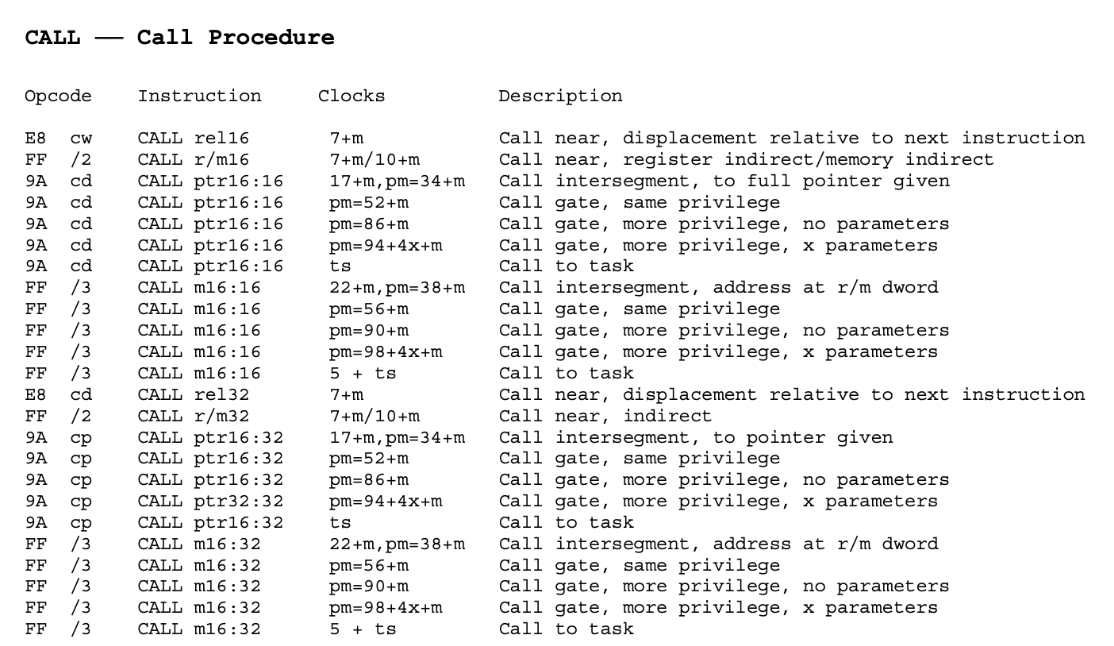
\includegraphics[scale=0.35]{fig/2.png}
        \caption{call-e8-J}
        \end{minipage}%
        \hfill
        \begin{minipage}[h]{0.5\linewidth}
        \centering
        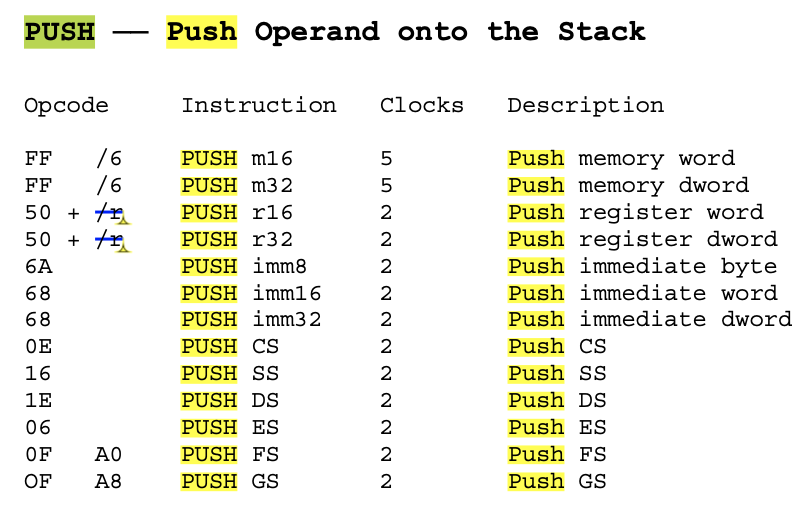
\includegraphics[scale=0.35]{fig/3.png}
        \caption{push-55-r}
        \end{minipage}
    \end{figure}
    \begin{figure}[!h]
        \begin{minipage}[h]{0.5\linewidth}
        \centering
        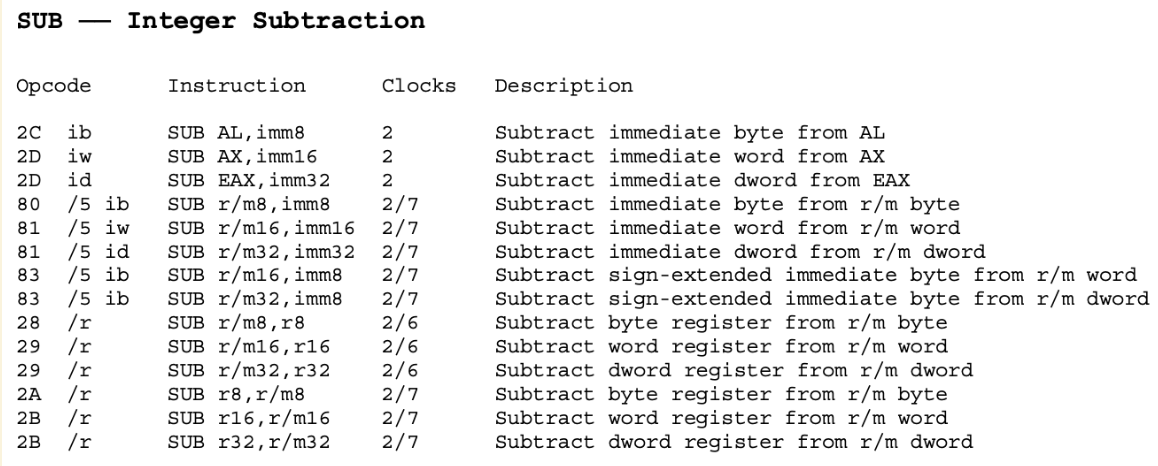
\includegraphics[scale=0.35]{fig/4.png}
        \caption{sub-83-gp1-6}
        \end{minipage}%
        \hfill
        \begin{minipage}[h]{0.5\linewidth}
        \centering
        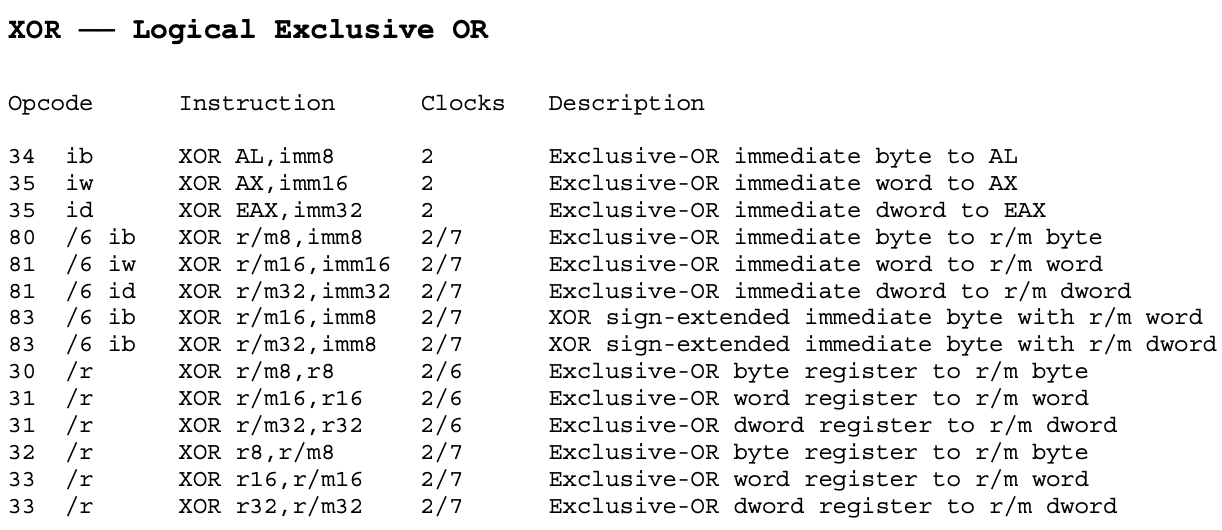
\includegraphics[scale=0.35]{fig/5.png}
        \caption{xor-31-G2E}
        \end{minipage}
    \end{figure}
    \begin{figure}[!h]
        \begin{minipage}[h]{0.5\linewidth}
        \centering
        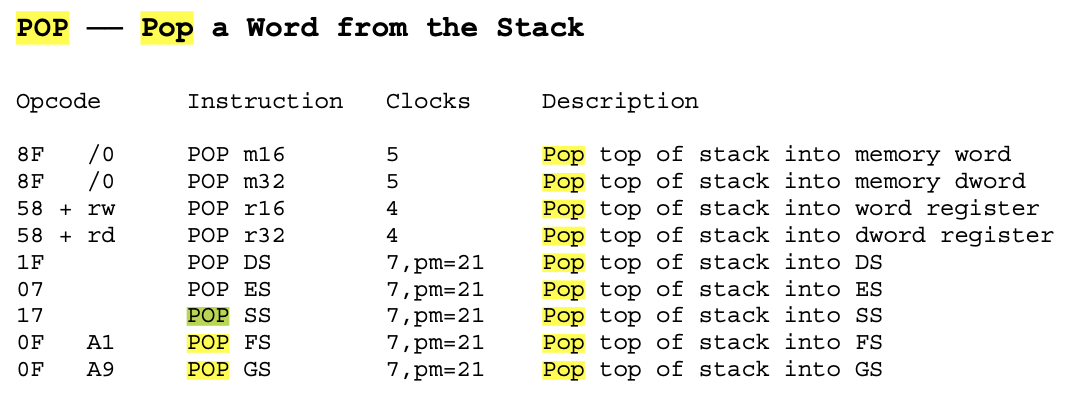
\includegraphics[scale=0.35]{fig/6.png}
        \caption{pop-5d-r}
        \end{minipage}%
        \hfill
        \begin{minipage}[h]{0.5\linewidth}
        \centering
        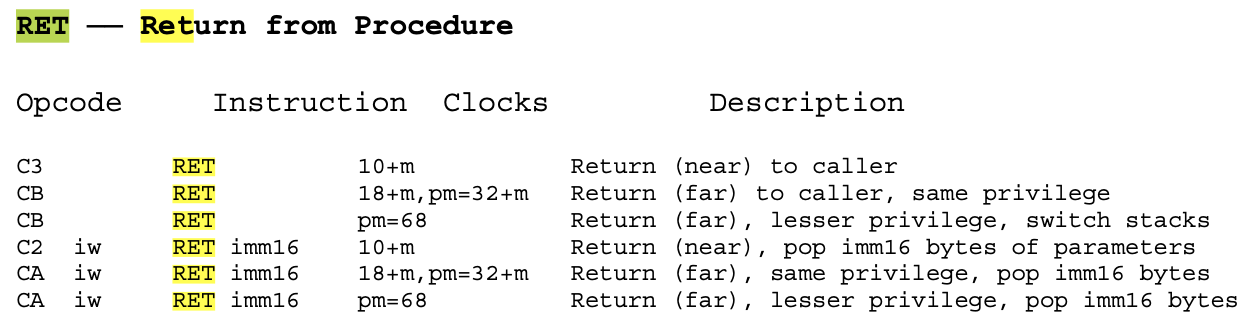
\includegraphics[scale=0.35]{fig/7.png}
        \caption{ret-c3}
        \end{minipage}
    \end{figure}
    根据上述RTFM结果,call指令的译码函数J($cpu.jmp_eip$=eip+SI),执行函数call,操作数宽度2/4,不设置宽度,所以在0xe8的位置填入IDEX(J,call),之后根据报错一步步实现符号立即数处理(SI),以及$rtl_push$和$rtl_sext$即可。
    \begin{lstlisting}[title=call指令实现,frame=trbl,language={C++}]
//nemu/src/cpu/exec/exec.c
/* 0xe8 */	IDEX(J,call), 
//nemu/src/cpu/exec/allinstr.h
/*control.c*/
make_EHelper(call);
//nemu/include/cpu/rtl.h
static inline void rtl_push(const rtlreg_t* src1) {
	rtl_subi(&cpu.esp,&cpu.esp,4);//esp-=4
	rtl_sm(&cpu.esp,src1,4);//src1写入esp
}
static inline void rtl_sext(rtlreg_t* dest, const rtlreg_t* src1, int width) {
  rtl_shli(dest, src1, 32 - width * 8);
  rtl_sari(dest, dest, 32 - width * 8);
}
//nemu/src/cpu/decode/decode.c
static inline make_DopHelper(SI) {
    assert(op->width == 1 || op->width == 4);
    op->type = OP_TYPE_IMM;
    op->simm = 1; //初始化
	t0 = instr_fetch(eip, op->width);//读指令
	rtl_sext(&t0, &t0, op->width);取SI
	op->simm = t0;//赋值
	//Log("fetch simm: %d", op->simm);
    //TODO();
    rtl_li(&op->val, op->simm);
#ifdef DEBUG
  snprintf(op->str, OP_STR_SIZE, "$0x%x", op->simm);
#endif
}
//nemu/src/cpu/exec/control.c
make_EHelper(call) {
    rtl_push(eip);//压栈eip
    rtl_j(decoding.jmp_eip);//跳转
    print_asm("call %x", decoding.jmp_eip);
}
    \end{lstlisting}

    push指令的译码函数r(读寄存器的值并存入op->val),执行函数push,操作数宽度2/4,不设置宽度,所以在0x50-0x57的位置填入IDEX(r,push),由于$rtl\_push$在call指令中已实现,之后声明并实现执行函数即可
    \begin{lstlisting}[title=push指令实现,frame=trbl,language={C++}]
//nemu/src/cpu/exec/exec.c
/* 0x50 */	IDEX(r,push), IDEX(r,push), IDEX(r,push), IDEX(r,push),
/* 0x54 */	IDEX(r,push), IDEX(r,push), IDEX(r,push), IDEX(r,push),
//nemu/src/cpu/exec/allinstr.h
/*data-mov.c*/
make_EHelper(push);
//nemu/src/cpu/exec/data-mov.c
make_EHelper(push) {
    //TODO();
    rtl_push(&id_dest->val);
    print_asm_template1(push);
}
    \end{lstlisting}

    sub指令的译码函数I2a(读eax中数据到dest,读立即数写入src),执行函数sub,/5表示填写在gp1的第六个位置即可,EX(sub),在reg.h中补上标志位的相关声明,在rtl.h中实现$rtl\_msb$以及一系列设置标志位的函数及相关宏再在arith.c中实现执行函数sub即可
    \begin{lstlisting}[title=sub指令实现,frame=trbl,language={C++}]
//nemu/src/cpu/exec/exec.c
/* 0x80, 0x81, 0x83 */
make_group(gp1,
    EX(add), EX(or), EX(adc), EX(sbb),
    EX(and), EX(sub),EX(xor), EX(cmp))
//nemu/include/cpu/reg.h
struct {
		rtlreg_t CF:1;rtlreg_t one1:1;
		rtlreg_t PF:1;rtlreg_t zero1:1;
	    rtlreg_t AF:1;rtlreg_t zero2:1;
		rtlreg_t ZF:1;rtlreg_t SF:1;
		rtlreg_t TF:1;rtlreg_t IF:1;
		rtlreg_t DF:1;rtlreg_t OF:1;
		rtlreg_t IOPL:2;rtlreg_t NT:1;
		rtlreg_t zero3:1;rtlreg_t RF:1;
		rtlreg_t VM:1;rtlreg_t zero:16;	
    }eflags;
//nemu/include/cpu/rtl.h
static inline void rtl_msb(rtlreg_t* dest, const rtlreg_t* src1, int width) {
    rtl_shri(dest, src1, width*8 - 1);//获取符号位
}
//设置获取标志位
#define make_rtl_setget_eflags(f) \
  static inline void concat(rtl_set_, f) (const rtlreg_t* src) { \
    cpu.eflags.f = *src; \
  } \
  static inline void concat(rtl_get_, f) (rtlreg_t* dest) { \
		*dest = cpu.eflags.f; \
  }
static inline void rtl_update_ZF(const rtlreg_t* result, int width) {
	rtl_shli(&at, result, 32 - width * 8);
	if(at == 0) cpu.eflags.ZF = 1;//是0则ZF标记1
	else cpu.eflags.ZF = 0;
}

static inline void rtl_update_SF(const rtlreg_t* result, int width) {
	rtl_msb(&at, result, width);//获取符号位
	cpu.eflags.SF = at;	
}
//nemu/src/cpu/exec/allinstr.h
/*arith.c*/
make_EHelper(sub);
//nemu/src/cpu/exec/arith.c
make_EHelper(sub) {//参考sbb代码并删除CF部分
  rtl_sub(&t2, &id_dest->val, &id_src->val);
  rtl_setrelop(RELOP_LTU, &t3, &id_dest->val, &t2);
  operand_write(id_dest, &t2);
  rtl_update_ZFSF(&t2, id_dest->width);
  //CF=1?进位
  rtl_setrelop(RELOP_LTU, &t0, &id_dest->val, &t2);
  rtl_or(&t0, &t3, &t0);
  rtl_set_CF(&t0);
  //OF溢出
  rtl_xor(&t0, &id_dest->val, &id_src->val);
  rtl_xor(&t1, &id_dest->val, &t2);
  rtl_and(&t0, &t0, &t1);
  rtl_msb(&t0, &t0, id_dest->width);
  rtl_set_OF(&t0);
//Log("%x-%x=%x",id_dest->val+id_src->val,id_src->val,id_dest->val);	

  print_asm_template2(sub);
}
    \end{lstlisting}

    xor指令的译码函数G2E,执行函数xor,操作数宽度2/4,不设置宽度,所以在0x31的位置填入IDEX(G2E,xor),之后声明并实现执行函数即可
    \begin{lstlisting}[title=xor指令实现,frame=trbl,language={C++}]
//nemu/src/cpu/exec/exec.c
/* 0x30 */	IDEXW(G2E,xor,1), IDEX(G2E,xor),
//nemu/src/cpu/exec/allinstr.h
/*logic.c*/
make_EHelper(xor);
//nemu/src/cpu/exec/logic.c
make_EHelper(xor) {
  //TODO();
  rtl_xor(&id_dest->val, &id_dest->val, &id_src->val);
  operand_write(id_dest,&id_dest->val);
  rtl_li(&t0,0);//t0=0  CF=OF=0
  rtl_set_CF(&t0);
  rtl_set_OF(&t0);
  rtl_update_ZFSF(&id_dest->val, id_dest->width);

  print_asm_template2(xor);
}
     \end{lstlisting}

     pop指令的译码函数r,执行函数pop,操作数宽度2/4,不设置宽度,所以在0x5d的位置填入IDEX(r,pop),并在rtl.h中实现$rtl\_pop$之后声明实现执行函数即可
    \begin{lstlisting}[title=pop指令实现,frame=trbl,language={C++}]
//nemu/src/cpu/exec/exec.c
/* 0x5c */	IDEX(r,pop), IDEX(r,pop),
//nemu/include/cpu/rtl.h
static inline void rtl_pop(rtlreg_t* dest) {
	rtl_lm(dest,&cpu.esp,4);
	rtl_addi(&cpu.esp,&cpu.esp,4);//esp+=4
}
//nemu/src/cpu/exec/allinstr.h
/*data-mov.c*/
make_EHelper(pop);
//nemu/src/cpu/exec/data-mov.c
make_EHelper(pop) {
  //TODO();
  rtl_pop(&id_src->val);
  operand_write(id_dest,&id_src->val);//写dest

  print_asm_template1(pop);
}
     \end{lstlisting}

     ret指令无译码函数,执行函数ret,所以在0xc3的位置填入EX(ret),之后声明实现执行函数即可
    \begin{lstlisting}[title=ret指令实现,frame=trbl,language={C++}]
//nemu/src/cpu/exec/exec.c
/* 0xc0 */
IDEXW(gp2_Ib2E, gp2,1),IDEX(gp2_Ib2E,gp2),IDEXW(I,ret,2),EX(ret),
//nemu/src/cpu/exec/allinstr.h
/*control.c*/
make_EHelper(ret);
//nemu/src/cpu/exec/control.c
make_EHelper(ret) {
    //TODO();
	rtl_pop(&decoding.jmp_eip);
	rtl_j(decoding.jmp_eip);

    print_asm("ret");
}
     \end{lstlisting}

     对以上全部指令正确实现之后,就可以看到dummy的正确运行结果:
     \begin{figure}[H]
        \centering
        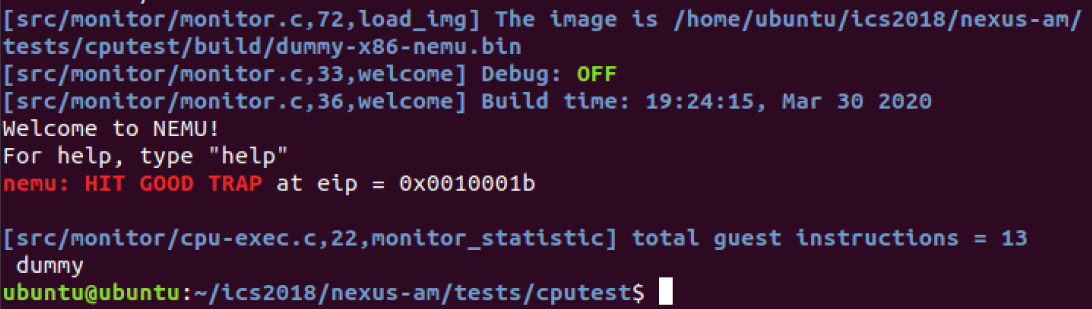
\includegraphics[scale=0.3]{fig/8.png}
        \caption{}
    \end{figure}
}  
%---------------------------------------------------------------------------------------------------
\section{阶段二}
%——————————————————————————————————————
\subsection{运行时环境、AM}
\kt{
    这一部分内容实际上是在说运行环境以及代码多样性导致的halt、trap等指令不同的解决方法——封装成库函数调用各自机器环境下的API,就好比PA1里面的$isa\_reg\_display$,由API在使用运行时环境提供相应功能。2018代码只有x86所以实际上没差。

    而AM就是使用这种API的抽象计算机。它提供运行时的环境,TRM部分就是PA1-PA2.2实现的提供计算能力的部分,IOE是要在PA2.3进行理解和解决的部分。CTE和VME见PA4。

    在了解了这一部分内容后,RTFSC整个代码结构就会变得容易许多。之后就是按照测试文件的顺序进行逐一实现。(PS:由于整体的实现过程与dummy大同小异,除特殊情况仅做代码和简单注释)
%——————————————————————————————————————
\subsection{add}
\kt{
    add中需要实现的指令是lea、and、nop、add、cmp、sete(setcc)、movzbl、test、je(jcc)、leave。
    \begin{lstlisting}[title=add,frame=trbl,language={C++}]
//nemu/src/cpu/exec/exec.c
/* 0x8c */	EMPTY, IDEX(lea_M2G,lea),
/* 0x80, 0x81, 0x83 */
make_group(gp1,
    EX(add), EX(or), EX(adc), EX(sbb),
    EX(and), EX(sub),EX(xor), EX(cmp))
/* 0x90 */	EX(nop),
/* 0x00 */
IDEXW(G2E,add,1),IDEX(G2E,add), IDEXW(E2G,add,1), IDEX(E2G,add),
/* 0x38 */	
IDEXW(G2E,cmp,1), IDEX(G2E,cmp), IDEXW(E2G,cmp,1), IDEX(E2G,cmp),
//0f对应的是2byte_esc所以要填第二张表查看i386手册90-9f都要填,movzbl同第二张表
/* 0x90 */	
IDEXW(setcc_E,setcc,1), IDEXW(setcc_E,setcc,1), IDEXW(setcc_E,setcc,1), IDEXW(setcc_E,setcc,1),
/* 0x94 */	
IDEXW(setcc_E,setcc,1), IDEXW(setcc_E,setcc,1), IDEXW(setcc_E,setcc,1), IDEXW(setcc_E,setcc,1),
/* 0x98 */	
IDEXW(setcc_E,setcc,1), IDEXW(setcc_E,setcc,1), IDEXW(setcc_E,setcc,1), IDEXW(setcc_E,setcc,1),
/* 0x9c */	
IDEXW(setcc_E,setcc,1), IDEXW(setcc_E,setcc,1), IDEXW(setcc_E,setcc,1), IDEXW(setcc_E,setcc,1),
/* 0xb4 */	EMPTY, EMPTY, IDEXW(mov_E2G,movzx,1),IDEXW(mov_E2G,movzx,2),
/* 0x84 */	IDEXW(G2E,test,1), IDEX(G2E,test),
/* 0x70 */	IDEXW(J,jcc,1), IDEXW(J,jcc,1), IDEXW(J,jcc,1), IDEXW(J,jcc,1),
/* 0x74 */	IDEXW(J,jcc,1), IDEXW(J,jcc,1), IDEXW(J,jcc,1), IDEXW(J,jcc,1),
/* 0x78 */	IDEXW(J,jcc,1), IDEXW(J,jcc,1), IDEXW(J,jcc,1), IDEXW(J,jcc,1),
/* 0x7c */	IDEXW(J,jcc,1), IDEXW(J,jcc,1), IDEXW(J,jcc,1), IDEXW(J,jcc,1),
//根据手册jcc需要将第一张表的70-7f以及0f对应的第二张表的80-8f都填上
/* 0x80 */	IDEX(J,jcc), IDEX(J,jcc), IDEX(J,jcc), IDEX(J,jcc),
/* 0x84 */	IDEX(J,jcc), IDEX(J,jcc), IDEX(J,jcc), IDEX(J,jcc),
/* 0x88 */	IDEX(J,jcc), IDEX(J,jcc), IDEX(J,jcc), IDEX(J,jcc),
/* 0x8c */	IDEX(J,jcc), IDEX(J,jcc), IDEX(J,jcc), IDEX(J,jcc),
/* 0xc8 */	EMPTY, EX(leave),
//nemu/src/cpu/exec/allinstr.h
/*data-mov.c*/
make_EHelper(lea);
make_EHelper(movzx);
make_EHelper(leave);
/*logic.c*/
make_EHelper(test);
make_EHelper(and);
make_EHelper(setcc);
/*special.c*/
make_EHelper(nop);
/*arith.c*/
make_EHelper(add);
make_EHelper(cmp);
/*control.c*/
make_EHelper(jcc);
//nemu/src/cpu/exec/data-mov.c
//lea和movzx已经实现了
make_EHelper(leave) {
  rtl_mv(&cpu.esp, &cpu.ebp);//esp=ebp
  rtl_pop(&cpu.ebp);	

  print_asm("leave");
}
//nemu/src/cpu/exec/logic.c
make_EHelper(test) {//and后不返回结果只设置标志位
  rtl_and(&t0, &id_dest->val, &id_src->val);
  rtl_update_ZFSF(&t0, id_dest->width);
  rtl_li(&t0,0);
  rtl_set_CF(&t0);
  rtl_set_OF(&t0);

  print_asm_template2(test);
}
make_EHelper(and) {
  rtl_and(&id_dest->val, &id_dest->val, &id_src->val);
  operand_write(id_dest, &id_dest->val);
  rtl_li(&t0,0);
  rtl_set_CF(&t0);
  rtl_set_OF(&t0);
  rtl_update_ZFSF(&id_dest->val, id_dest->width);

  print_asm_template2(and);
}
//虽然setcc的声明在logic里但实际需要实现的是cc.c里的rtl_setcc
//nemu/src/cpu/exec/cc.c--rtl_setcc
switch (subcode & 0xe) {//对i386手册内容翻译
    case CC_O:
      rtl_get_OF(&t0);*dest = t0 ? 1 : 0;break;
      //set byte if overflow (OF = 1)
    case CC_B:
      rtl_get_CF(&t0);*dest = t0 ? 1 : 0;break;
      //set byte if below (CF = 1)
    case CC_E:
      rtl_get_ZF(&t0);*dest = t0 ? 1 : 0;break;
      //set byte if equal (ZF = 1)
    case CC_BE:
      rtl_get_ZF(&t0);rtl_get_CF(&t1);*dest = (t0 || t1) ? 1 : 0;break;
      //set byte if below or equal (CF = 1 or ZF = 1)
    case CC_S:
      rtl_get_SF(&t0);*dest = t0 ? 1 : 0;break;
      /set byte if sign (SF = 1) 	
    case CC_L:
      rtl_get_SF(&t0);rtl_get_OF(&t1);*dest = (t0 != t1) ? 1 : 0;break;
      //set byte if less (SF != OF)
    case CC_LE:
      rtl_get_SF(&t0);rtl_get_OF(&t1);
      rtl_get_ZF(&t2);*dest = ((t0 != t1) || t2) ? 1 : 0;break;
      //set byte if less or equal (ZF = 1 or SF != OF)
      //TODO();
    default: panic("should not reach here");
    case CC_P: panic("n86 does not have PF");
}
//nop不需要写--因为本身就是 no operation的意思
//nemu/include/cpu/rtl.h
static inline void rtl_not(rtlreg_t *dest, const rtlreg_t* src1) {
    *dest=~(*src1);
}
//nemu/src/cpu/exec/arith.c
make_EHelper(add) {//参考adc删去CF两句
  rtl_add(&t2, &id_dest->val, &id_src->val);
  rtl_setrelop(RELOP_LTU, &t3, &t2, &id_dest->val);
  operand_write(id_dest, &t2);
  rtl_update_ZFSF(&t2, id_dest->width);
  rtl_setrelop(RELOP_LTU, &t0, &t2, &id_dest->val);
  rtl_or(&t0, &t3, &t0);
  rtl_set_CF(&t0);
  rtl_xor(&t0, &id_dest->val, &id_src->val);
  rtl_not(&t0, &t0);
  rtl_xor(&t1, &id_dest->val, &t2);
  rtl_and(&t0, &t0, &t1);
  rtl_msb(&t0, &t0, id_dest->width);
  rtl_set_OF(&t0);

  print_asm_template2(add);
}
make_EHelper(cmp) {
  rtl_sub(&t2, &id_dest->val, &id_src->val);//相减
  rtl_setrelop(RELOP_LTU, &t3, &id_dest->val, &t2);//dest<t2?
  rtl_update_ZFSF(&t2, id_dest->width);
  rtl_setrelop(RELOP_LTU, &t0, &id_dest->val, &t2);
  rtl_or(&t0, &t3, &t0);
  rtl_set_CF(&t0);
  rtl_xor(&t0, &id_dest->val, &id_src->val);
  rtl_xor(&t1, &id_dest->val, &t2);
  rtl_and(&t0, &t0, &t1);
  rtl_msb(&t0, &t0, id_dest->width);//符号位看溢出
  rtl_set_OF(&t0);

  print_asm_template2(cmp);
}
//jcc也已实现执行函数
    \end{lstlisting}

}
%——————————————————————————————————————
\subsection{add-longlong}
\kt{
    add-longlong只需实现adc和or在opcode\_table中的部分以及or的执行函数
    \begin{lstlisting}[title=add-longlong,frame=trbl,language={C++}]
//nemu/src/cpu/exec/exec.c 
/* 0x10 */	IDEXW(G2E,adc,1),IDEX(G2E,adc),IDEXW(E2G,adc,1),IDEX(E2G,adc),
/* 0x08 */  IDEXW(G2E,or,1), IDEX(G2E,or),
//nemu/src/cpu/exec/logic.c 
  rtl_or(&id_dest->val, &id_dest->val, &id_src->val);	
  operand_write(id_dest, &id_dest->val);	
  rtl_li(&t0,0);
  rtl_set_CF(&t0);
  rtl_set_OF(&t0);
  rtl_update_ZFSF(&id_dest->val, id_dest->width);

  print_asm_template2(or);
}
    \end{lstlisting}
}
%——————————————————————————————————————
\subsection{bit、bubble-sort}
\kt{
    需要实现sar、shl、dec指令以及bubble-sort里的inc
    \begin{lstlisting}[title=bit,frame=trbl,language={C++}]
//nemu/src/cpu/exec/exec.c 
/* 0xc0, 0xc1, 0xd0, 0xd1, 0xd2, 0xd3 */
make_group(gp2,
    EX(rol), EMPTY, EMPTY, EMPTY,
    EX(shl), EX(shr), EMPTY, EX(sar))
/* 0xfe */
make_group(gp4,
    EX(inc), EX(dec), EMPTY, EMPTY,
    EMPTY, EMPTY, EMPTY, EMPTY)
/* 0x40 */	IDEX(r,inc), IDEX(r,inc), IDEX(r,inc), IDEX(r,inc),
//nemu/src/cpu/exec/logic.c 
make_EHelper(sar) {
  rtl_sext(&id_dest->val, &id_dest->val, id_dest->width);//取符号
  rtl_sar(&id_dest->val, &id_dest->val, &id_src->val);
  operand_write(id_dest, &id_dest->val);
  rtl_update_ZFSF(&id_dest->val, id_dest->width);

  print_asm_template2(sar);
}
make_EHelper(shl) {
  rtl_shl(&id_dest->val, &id_dest->val, &id_src->val);
  operand_write(id_dest, &id_dest->val);
  rtl_update_ZFSF(&id_dest->val, id_dest->width);

  print_asm_template2(shl);
}
//nemu/src/cpu/exec/arith.c 
make_EHelper(dec) {
  rtl_subi(&t2, &id_dest->val, 1);
  rtl_setrelop(RELOP_LTU, &t3, &id_dest->val, &t2);
  operand_write(id_dest, &t2);
  rtl_update_ZFSF(&t2, id_dest->width);
  rtl_setrelop(RELOP_LTU, &t0, &id_dest->val, &t2);
  rtl_or(&t0, &t3, &t0);
  rtl_xori(&t0, &id_dest->val, 1);
  rtl_xor(&t1, &id_dest->val, &t2);
  rtl_and(&t0, &t0, &t1);
  rtl_msb(&t0, &t0, id_dest->width);
  rtl_set_OF(&t0);

  print_asm_template1(dec);
}
make_EHelper(inc) {
  rtl_addi(&t2, &id_dest->val,1);
  rtl_setrelop(RELOP_LTU, &t3, &t2, &id_dest->val);
  operand_write(id_dest, &t2);
  rtl_update_ZFSF(&t2, id_dest->width);
  rtl_setrelop(RELOP_LTU, &t0, &t2, &id_dest->val);
  rtl_or(&t0, &t3, &t0);
  rtl_xori(&t0, &id_dest->val, 1);
  rtl_not(&t0, &t0);
  rtl_xor(&t1, &id_dest->val, &t2);
  rtl_and(&t0, &t0, &t1);
  rtl_msb(&t0, &t0, id_dest->width);
  rtl_set_OF(&t0);

  print_asm_template1(inc);
}
    \end{lstlisting}
}
%——————————————————————————————————————
\subsection{其他指令}
\kt{
    imul、cltd、idiv、jmp、shr、sbb
    \begin{lstlisting}[title=余下指令,frame=trbl,language={C++}]
//nemu/src/cpu/exec/exec.c   
/* 0xf6, 0xf7 */
make_group(gp3,
    IDEX(test_I,test), EMPTY, EX(not), EX(neg),
    EX(mul), EX(imul1), EX(div), EX(idiv))
/* 0x68 */	IDEX(push_SI,push), IDEX(I_E2G,imul3), IDEXW(push_SI,push,1), IDEXW(I_E2G,imul3,1), 
/* 0x98 */	EX(cwtl), EX(cltd),
/* 0x18 */	IDEXW(G2E,sbb,1), IDEX(G2E,sbb), IDEXW(E2G,sbb,1), IDEX(E2G,sbb),
//nemu/src/cpu/exec/data-mov.c
make_EHelper(cltd) {//引用
  if (decoding.is_operand_size_16) {//16b
  rtl_sext(&t0,&reg_l(R_EAX),2);//EAX的符号位
  rtl_mv(&reg_l(R_EDX), (&t0)+2);//到edx中变为双长
  }
  else {
  rtl_sari(&reg_l(R_EDX), &reg_l(R_EAX), 31);//符号位扩展到edx
  }
//nemu/src/cpu/exec/logic.c
make_EHelper(shr) {
  rtl_shr(&id_dest->val, &id_dest->val, &id_src->val);
  operand_write(id_dest, &id_dest->val);
  rtl_update_ZFSF(&id_dest->val, id_dest->width);

  print_asm_template2(shr);
}
    \end{lstlisting}  

}

确保全部指令实现正确(monitor返回good\ trap)后就可以通过测试样例了,但是其实好多指令并没有实现(TODO遍布在NEMU的每一个角落)但是可以继续往下实现常用库函数
%——————————————————————————————————————
\subsection{字符串处理函数}
实在是想不到有一天我一个用都用不熟的人还要来实现它本身(实现了一下发现其实比用起来简单),那就只能借助man命令的RTFM和STFW实现了。整体不是很难,基本上只要弄清楚这个函数的用途以及字符串本身特征还有数据类型转换正确等等就可以了。
\begin{lstlisting}[title=string.c,frame=trbl,language={C++}]
//nexus-am/libs/klib/src/string.c  
size_t strlen(const char *s) {
  size_t i = 0;//遇到结束符\0之前统计字符个数即可
  while(*(s + i) != '\0')
    i ++;
  return i;
} 
char *strcpy(char* dst,const char* src) {
  int i = 0;//逐个复制
  while(*(src + i) != '\0'){
    *(dst + i) = *(src + i);
    i ++;
  }
  return dst;
}
char* strncpy(char* dst, const char* src, size_t n) {
  size_t i;//规定长度加上限制,同时不能忘了在最后加上\0
  for(i = 0; i < n && src[i] != '\0'; ++i)
    dst[i] = src[i];
  for( ; i < n; ++i)
    dst[i] = '\0';
  return dst;
}
char* strcat(char* dst, const char* src) {
  size_t dst_len = strlen(dst);//拼接即可
  size_t i = 0;
  for(i = 0; src[i] != '\0'; ++i)
    dst[dst_len + i] = src[i];
  dst[dst_len + i] = '\0';
  return dst;
}
int strcmp(const char* s1, const char* s2) {
  int len1 = strlen(s1),len2 = strlen(s2),len = 0;
  if(len1 < len2) len = len1;//比对到短的即可
  else len = len2;
  for(int i = 0; i <= len; ++i){
    if(s1[i] < s2[i]) return -1;
    else if(s1[i] > s2[i]) return 1;
  }
  return 0;//一样
}
int strncmp(const char* s1, const char* s2, size_t n) {
  for(size_t i = 0; i < n; ++i){//最多比较前n个字符
    if(s1[i] < s2[i]) return -1;
    else if(s1[i] > s2[i]) return 1;
  }
  return 0;
}
void* memset(void* v,int c,size_t n) {
  if(v == NULL || n < 0) return NULL;
  char* temp = (char*) v;
  for(int i = 0; i < n; ++i)
    temp[i] = (char) c;//按ASCII全体赋值
  return v;
}
void* memcpy(void* out, const void* in, size_t n) {
  if(out == NULL || n < 0) return NULL;
  char* chardest = (char*) out;
  char* charsrc = (char*) in;
  for(int i = 0; i < n; ++i)
    chardest[i] = charsrc[i];//copy
  return out;
}

int memcmp(const void* s1, const void* s2, size_t n){
  char* ch1 = (char*) s1;//同strcmp理
  char* ch2 = (char*) s2;
  for(int i = 0; i < n; ++i){
    if(ch1[i] < ch2[i]) return -1;
    else if(ch1[i] > ch2[i]) return 1;
  }
  return 0;
}
\end{lstlisting}

将string.c实现之后运行string测试样例即可得到good trap结果
%——————————————————————————————————————
\subsection{标准输入输出}
之后需要实现stdio.c中的标准输入输出才可以使hello-str通过(既然迟早都得实现为什么不干脆一次性实现完)。就像PA2.3里提及的sprintf和printf的代码会有较大的重叠,即他们都有和vsprintf实现内容重叠的部分,所以先实现vsprintf之后再调用实现sprintf和printf
\begin{lstlisting}[title=stdio.c,frame=trbl,language={C++}]
//nexus-am/libs/klib/src/stdio.c 
int vsprintf(char *out, const char *fmt, va_list ap) {
  char *outp;
  nt out_len=0;
  int width;//宽度
  int flags;//标记
  char nums[1000];
  char *ss=nums;
  for(outp=out;*fmt;fmt++){
    if(*fmt!='%'){//计数
      *outp++=*fmt;
      out_len++;
      continue;
    }
    int temp=1;//处理flags
    flags=0;
    while(temp==1){
      fmt++;
      switch(*fmt){
        case '0':flags|=1;break;//左边置0
        case '+':flags|=4;break;//显示正负号
        case ' ':flags|=8;break;//插入空格
        case '-':flags|=16;break;//左对齐
        case '#':flags|=32;break;//0x.
        default:temp=0;
      }
    }
    width=0;//处理宽度
    if(*fmt>='0'&&*fmt<='9'){
      for(;*fmt>='0'&&*fmt<='9';fmt++){
        width=width*10+*fmt-'0';//编译原理处理方法
      }
    }
    else if(*fmt=='*'){
      fmt++;
      width=va_arg(ap,int);//在ap里找下一个int型
      if(width<0){
        width=-width;
        flags|=16;
      }
    }
    switch(*fmt){
      case 'd':break;
      case 's':{
        char *s=va_arg(ap,char *);
        int len_s=strlen(s);
        if(!(flags&16)){//默认右对齐
          while(len_s<width--){//不足width的填空格
            *outp++=' ';out_len++;
          }
        }
        for(int i=0;i<len_s;i++){
          *outp++=*s++;out_len++;
        }
        while(len_s<width--){//补空格到width
          *outp++=' ';out_len++;
        }
        continue;
      }
    }

    int num=va_arg(ap,int);
    int count=0;
    if(num==0){
      *ss++='0';
      count+=1;
    }
    else{
      if(num<0){//负号
        *outp++='-';out_len++;
        num=-num;
      }
      while(num){
        *ss++=num%10+'0';//转str
        num=num/10;
        count+=1;
      }
    }
    if(count<width){
      num=width-count;
      if(flags&1){//flags0
        while(num--){
          *outp++='0';out_len++;
        }
      }
      else if(flags&8){//flags ' '
        while(num--){
          *outp++=' ';out_len++;
        }
      }
    }
    while(count--){
      *outp++=*--ss;out_len++;
    }
  } 
  *outp='\0';
  return out_len;//返回写入的字符总数
}
int sprintf(char *out, const char *fmt, ...) {
  va_list args;
  va_start(args,fmt);//实际上就是调用vsprintf把args替换到fmt里面存到out
  int out_len=vsprintf(out,fmt,args);
  va_end(args);
  return out_len;
}
int printf(const char *fmt, ...) {
  va_list args;
  va_start(args,fmt);
  char out[1000];
  int out_len=vsprintf(out,fmt,args);
  va_end(args);
  for(int i=0;i<out_len;i++){
    //nexus-am/am/arch/x86-nemu/src/trm.c中
    _putc(out[i]);//使用_putc输出由于串口未实现所以此时并不可以正确输出
  }
  return 0;
}
\end{lstlisting} 

实现完stdio.c之后再进行hello-str的测试就可以正常通过了,此时使用后文提及的回归测试所用的bash脚本runall.sh即可测出正常通过测试。
\begin{figure}[H]
    \centering
    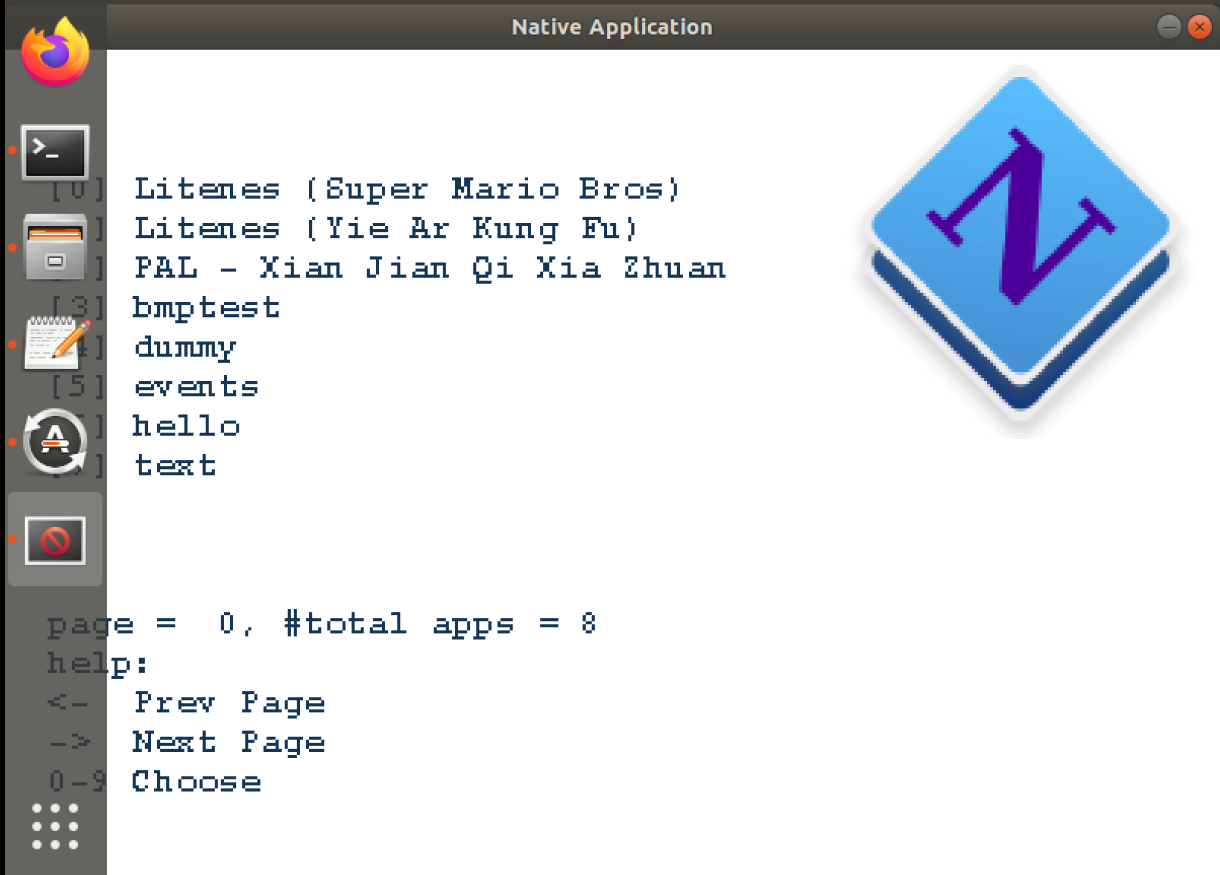
\includegraphics[scale=0.25]{fig/9.jpeg}
    \caption{runall.sh}
\end{figure}
%——————————————————————————————————————
\subsection{Differential Testing}
\kt{
    这里的DiffTest虽然放在了PA2.2的末尾但是作为基础设施!它应该在PA2.1至少2.2的开头实现,不然真的难以de那些奇奇怪怪的错,光靠native上跑一个没有输出的测试样例是正确的显然不行,借助DiffTest和Qemu进行一步一步的对比就可以更快的找出错在哪里,尤其是标志位出错,大部分出错都和标志位还有寄存器的写有关,再者是逐步执行并比对,所以可以更准确的定位错误,所以虽然在章节的末尾,实际上我在2.2疯狂报错找不出原因以后就开始写了。
    
    在common.h中定义DiffTest并实现difftest\_step中DiffTest的核心功能即可
    \begin{lstlisting}[title=DiffTest,frame=trbl,language={C++}]
//nemu/src/monitor/difftest/difftest.c
//代码框架中载入QEMU并连接逐步执行都已经实现,只需要把reg的检查补充完整就好
bool diff=false;//确有不同
if(ref_r.eip != cpu.eip){
      diff = true;
      printf("Diff: eip  QEMU: 0x%08x\n",ref_r.eip);
      printf("           NEMU: 0x%08x\n",cpu.eip);
  }
  if(ref_r.eax != cpu.eax){
      diff = true;
      printf("Diff: eax  QEMU: 0x%08x\n",ref_r.eax);
      printf("           NEMU: 0x%08x\n",cpu.eax);
  }
  if(ref_r.ecx != cpu.ecx){
      diff = true;
      printf("Diff: ecx  QEMU: 0x%08x\n",ref_r.ecx);
      printf("           NEMU: 0x%08x\n",cpu.ecx);
  }
  if(ref_r.ebx != cpu.ebx){
      diff = true;
      printf("Diff: ebx  QEMU: 0x%08x\n",ref_r.ebx);
      printf("           NEMU: 0x%08x\n",cpu.ebx);
  }
  if(ref_r.edx != cpu.edx){
      diff = true;
      printf("Diff: edx  QEMU: 0x%08x\n",ref_r.edx);
      printf("           NEMU: 0x%08x\n",cpu.edx);
  }
  if(ref_r.ebp != cpu.ebp){
      diff = true;
      printf("Diff: ebp  QEMU: 0x%08x\n",ref_r.ebp);
      printf("           NEMU: 0x%08x\n",cpu.ebp);
  }
  if(ref_r.esp != cpu.esp){
      diff = true;
      printf("Diff: esp  QEMU: 0x%08x\n",ref_r.esp);
      printf("           NEMU: 0x%08x\n",cpu.esp);
  }
  if(ref_r.esi != cpu.esi){
      diff = true;
      printf("Diff: esi  QEMU: 0x%08x\n",ref_r.esi);
      printf("           NEMU: 0x%08x\n",cpu.esi);
  }
  if(ref_r.edi != cpu.edi){
      diff = true;
      printf("Diff: edi  QEMU: 0x%08x\n",ref_r.edi);
      printf("           NEMU: 0x%08x\n",cpu.edi);
  }
  if (diff) {//只比对NEMU有的标志位
    printf("ZF---NEMU:%d QEMU:%d\n",cpu.eflags.ZF,ref_r.eflags.ZF);
    printf("SF---NEMU:%d QEMU:%d\n",cpu.eflags.SF,ref_r.eflags.SF);
    printf("OF---NEMU:%d QEMU:%d\n",cpu.eflags.OF,ref_r.eflags.OF);
    printf("CF---NEMU:%d QEMU:%d\n",cpu.eflags.CF,ref_r.eflags.CF);
    printf("IF---NEMU:%d QEMU:%d\n",cpu.eflags.IF,ref_r.eflags.IF);
    nemu_state = NEMU_ABORT;//abort返回
  }
    \end{lstlisting}

}
}
%---------------------------------------------------------------------------------------------------
\section{阶段三}
%——————————————————————————————————————
\subsection{串口}
\kt{
    串口作为最简单的输入输出设备,基本的API都已经实现,只需要实现system.c中的in和out指令调用相应函数即可实现简单输入输出。实现参照port-io.c的pio\_read\_common和pio\_write\_common对宽度进行区分即可。
    \begin{lstlisting}[title=串口in\ out,frame=trbl,language={C++}]
//nemu/src/cpu/exec/system.c
make_EHelper(in) {//参照src/device/io/port-io.c
  switch(id_dest->width){
    case 4: rtl_li(&t0, pio_read_l(id_src->val)); break; 
    case 2: rtl_li(&t0, pio_read_w(id_src->val)); break; 
    case 1: rtl_li(&t0, pio_read_b(id_src->val)); break; 
  }
  operand_write(id_dest,&t0);

  print_asm_template2(in);

#if defined(DIFF_TEST)
  difftest_skip_ref();
#endif
}
make_EHelper(out) {
  switch(id_dest->width){
    case 4: pio_write_l(id_dest->val, id_src->val); break;
    case 2: pio_write_w(id_dest->val, id_src->val); break;
    case 1: pio_write_b(id_dest->val, id_src->val); break;
  }

  print_asm_template2(out);

#if defined(DIFF_TEST)
  difftest_skip_ref();
#endif
}
    \end{lstlisting}
    
    完成之后在nexus-am/apps/hello/下make\ run可以得到正确输出10次的Hello\ World!
    \begin{figure}[H]
        \centering
        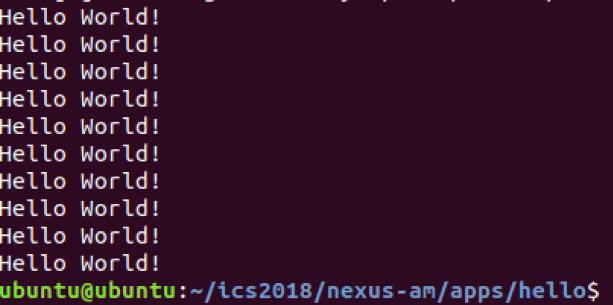
\includegraphics[scale=0.45]{fig/10.png}
        \caption{串口io}
    \end{figure}

}
%——————————————————————————————————————
\subsection{时钟}
\kt{
    时钟功能在timer.c里也被做了简化,只需要实现\_DEVREG\_TIMER\_UPTIME这一表示AM系统启动时间的寄存器内容更新即可
    \begin{lstlisting}[title=timer,frame=trbl,language={C++}]
//nexus-am/am/arch/x86-nemu/src/devices/timer.c
#define RTC_PORT 0x48
uint32_t boot_time;
void timer_init() {
	boot_time = inl(RTC_PORT);	
}
case _DEVREG_TIMER_UPTIME: {//case 1 hi和lo拼起来是最后的ms
    _UptimeReg *uptime = (_UptimeReg *)buf;
    uint64_t temptime = inl(RTC_PORT) - boot_time;//inl->uint32_t
    uptime->hi = (uint32_t) (temptime >> 32);//高32
    uptime->lo = (uint32_t) temptime;//低32
    return sizeof(_UptimeReg);
}
\end{lstlisting}

实现之后可以得到timetest每隔1s的输出:
\begin{figure}[H]
    \centering
    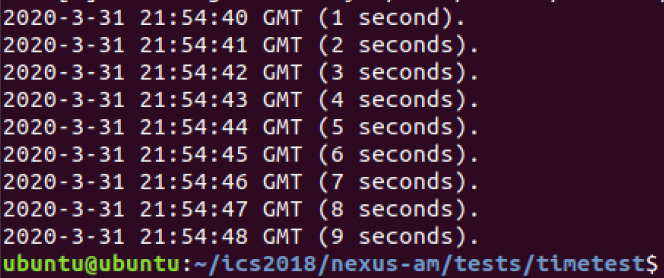
\includegraphics[scale=0.45]{fig/11.png}
    \caption{timer}
\end{figure}

关闭DEBUG和DIFFTEST宏之后对三个benchmark进行跑分测试:
\begin{figure}[!h]
    \begin{minipage}[h]{0.5\linewidth}
    \centering
    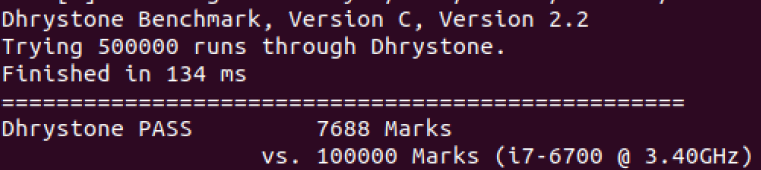
\includegraphics[scale=0.25]{fig/12.png}
    \caption{dhrystone-nemu}
    \end{minipage}%
    \hfill
    \begin{minipage}[h]{0.5\linewidth}
    \centering
    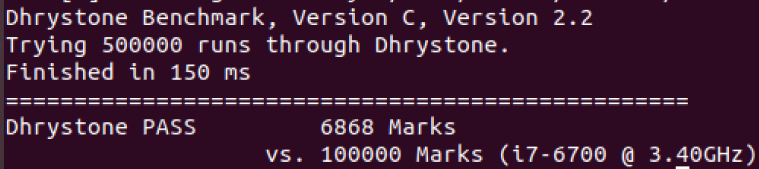
\includegraphics[scale=0.25]{fig/13.png}
    \caption{dhrystone-native}
    \end{minipage}
\end{figure}

\begin{figure}[!h]
    \begin{minipage}[h]{0.5\linewidth}
    \centering
    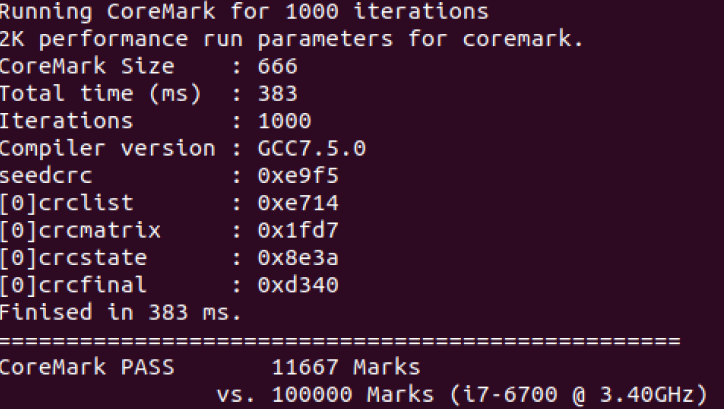
\includegraphics[scale=0.25]{fig/14.png}
    \caption{coremark-nemu}
    \end{minipage}%
    \hfill
    \begin{minipage}[h]{0.5\linewidth}
    \centering
    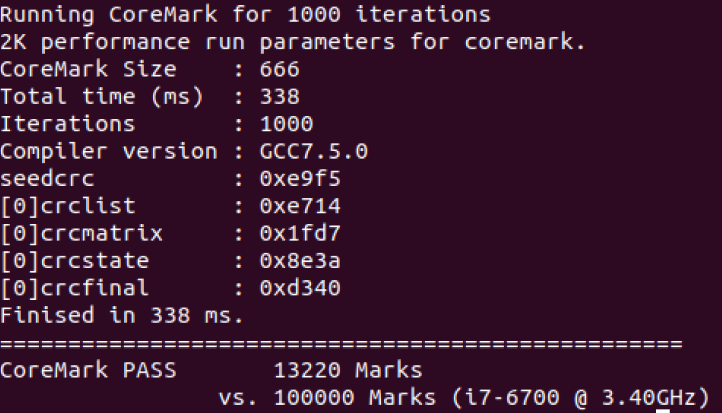
\includegraphics[scale=0.25]{fig/15.png}
    \caption{coremark-native}
    \end{minipage}
\end{figure}

\begin{figure}[!h]
    \begin{minipage}[h]{0.5\linewidth}
    \centering
    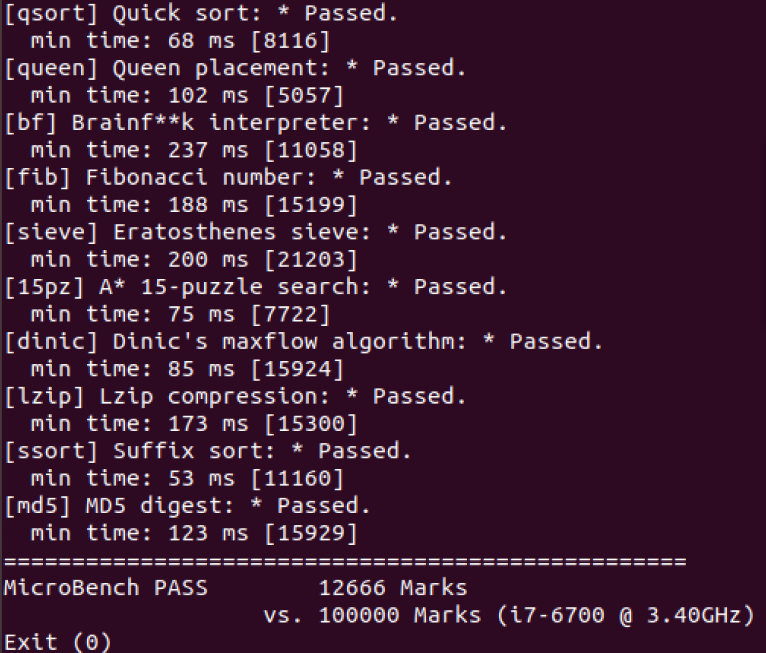
\includegraphics[scale=0.25]{fig/16.png}
    \caption{microbench-nemu}
    \end{minipage}%
    \hfill
    \begin{minipage}[h]{0.5\linewidth}
    \centering
    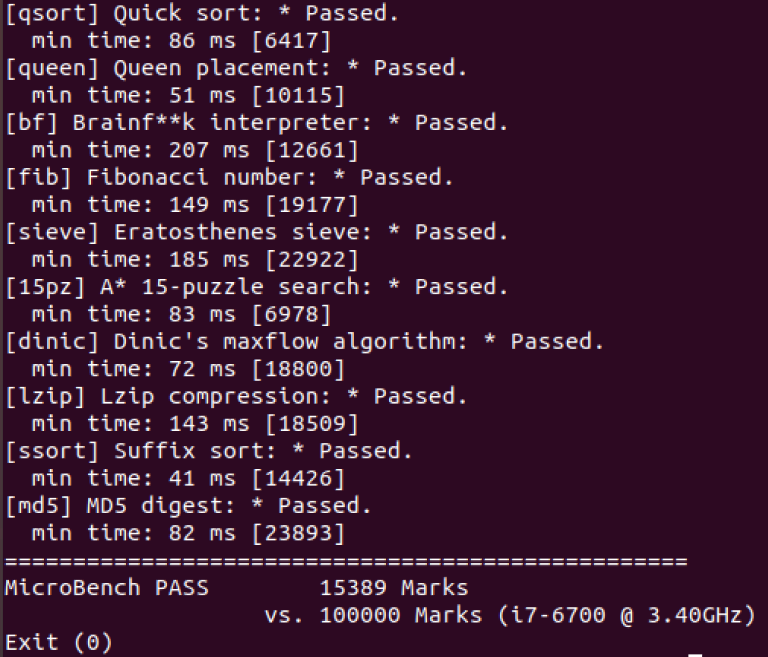
\includegraphics[scale=0.25]{fig/17.png}
    \caption{microbench-native}
    \end{minipage}
\end{figure}
}
%——————————————————————————————————————
\subsection{键盘}
\kt{
    键盘的按下检测在OS中实际上是一种中断,在NEMU中同样和上述外设一样还是有一个专用寄存器来完成读写的过程。
    \begin{lstlisting}[title=keyboard,frame=trbl,language={C++}]
//nexus-am/am/arch/x86-nemu/src/devices/input.c
#define I8042_DATA_PORT 0x60
case _DEVREG_INPUT_KBD: {
    _KbdReg *kbd = (_KbdReg *)buf;
    int keytemp = inl(I8042_DATA_PORT);//获取键盘码
    kbd->keydown = ((keytemp & 0x8000) == 0x8000) ? 1 : 0;//是否摁下
    kbd->keycode = keytemp;
    return sizeof(_KbdReg);
}
    \end{lstlisting}
    之后的keytest测试结果如下:
    \begin{figure}[H]
        \centering
        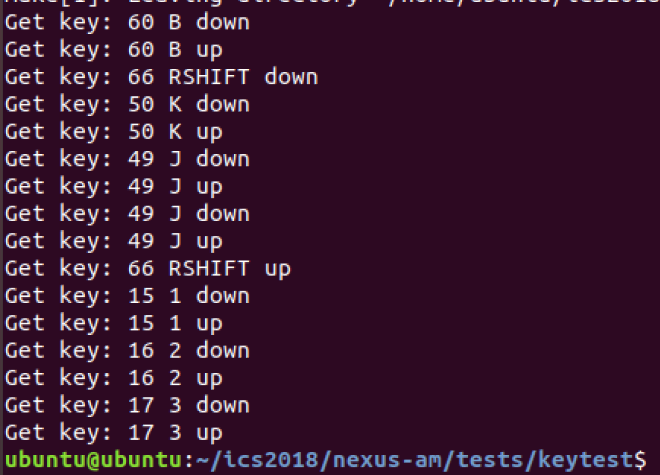
\includegraphics[scale=0.45]{fig/18.png}
        \caption{keyboard}
    \end{figure}
}
%——————————————————————————————————————
\subsection{VGA}
\kt{
    VGA设备需要实现屏幕大小信息给CPU的传递以及通过\_FBCtlReg结构体写入进行图像显示,同样是根据amdev.h中声明的成员变量进行传递赋值即可。
    \begin{lstlisting}[title=vga,frame=trbl,language={C++}]
//nexus-am/am/arch/x86-nemu/src/devices/video.c
#define SCREEN_PORT 0x100
#define SCREEN_H 300
#define SCREEN_W 400
case _DEVREG_VIDEO_INFO: {
    _VideoInfoReg *info = (_VideoInfoReg *)buf;
    info->width = SCREEN_W;
    info->height = SCREEN_H;
    return sizeof(_VideoInfoReg);
}
case _DEVREG_VIDEO_FBCTL: {
    _FBCtlReg *ctl = (_FBCtlReg *)buf;
	int x = ctl->x, y = ctl->y, w = ctl->w, h = ctl->h;
	uint32_t *pixels = ctl->pixels;
	int cp_bytes = sizeof(uint32_t) * min(w, SCREEN_W - x);
	for(int j = 0; j < h  && y + j < SCREEN_H; ++j){
		memcpy(&fb[(y + j) * SCREEN_W + x], pixels, cp_bytes);
	    pixels += w;
	}
    if (ctl->sync) {
        // do nothing, hardware syncs.
    }
      return sizeof(_FBCtlReg);
}
    \end{lstlisting}
    \begin{figure}[H]
        \centering
        
\includegraphics[scale=0.25]{fig/19.png}
        \caption{vga}
    \end{figure}

    全部IOE实现以后程序打字机和幻灯片就可以运行了,Mario也可以了
    \begin{figure}[H]
        \centering
        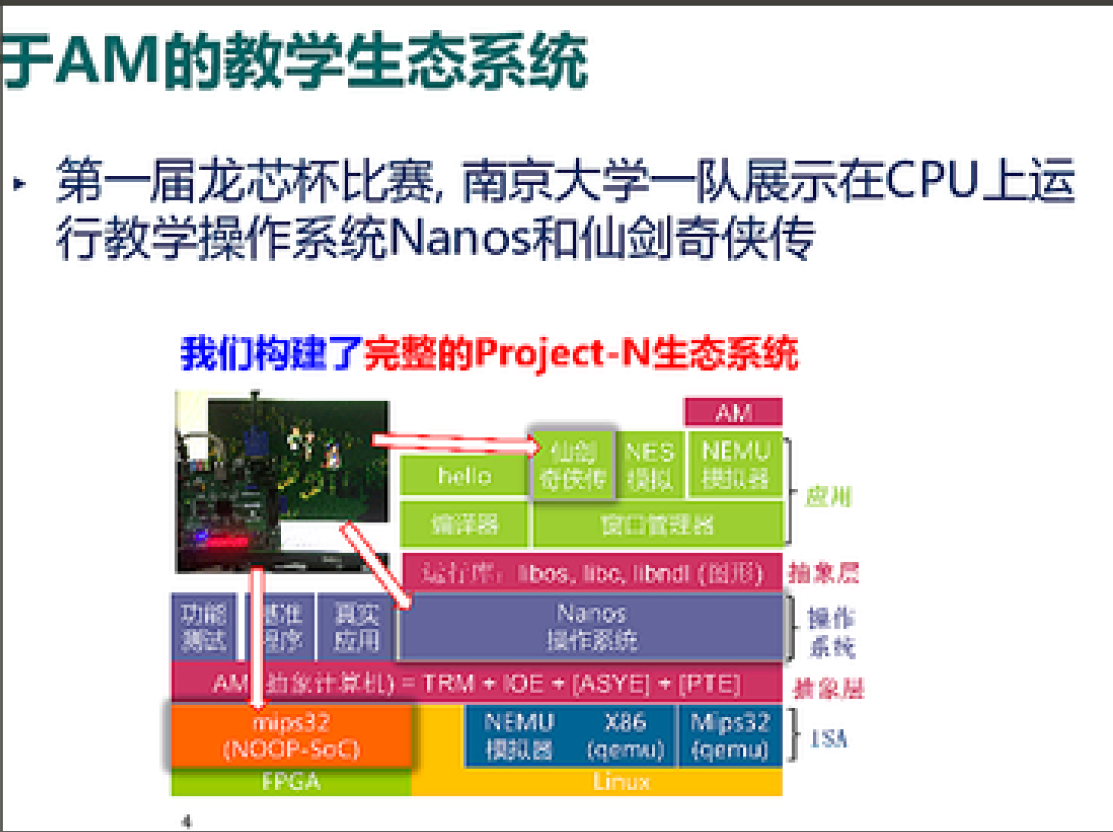
\includegraphics[scale=0.25]{fig/20.png}
        \caption{slider}
    \end{figure}
    \begin{figure}[H]
        \centering
        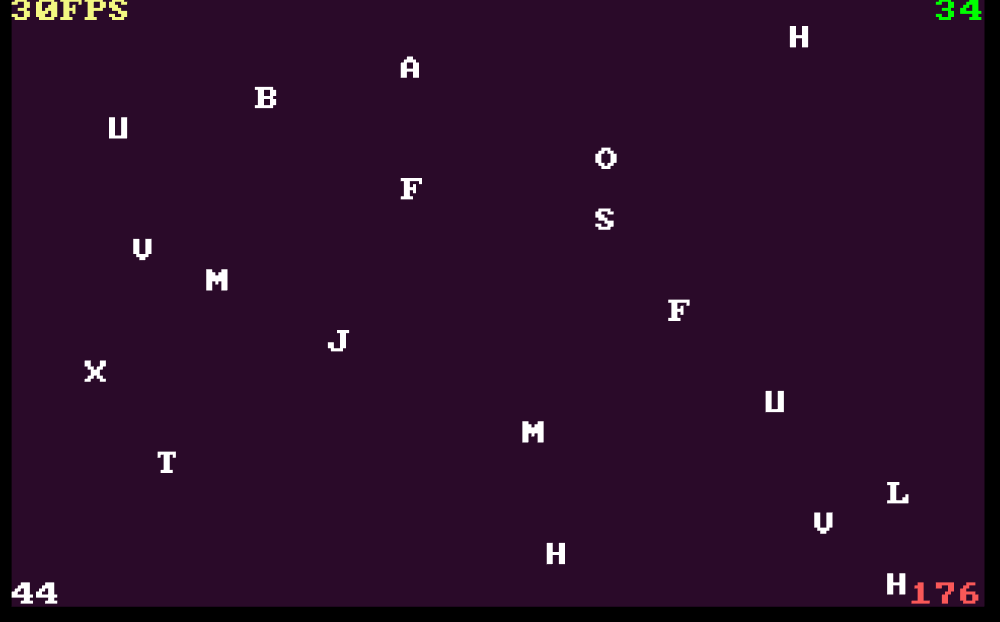
\includegraphics[scale=0.25]{fig/21.png}
        \caption{typing}
    \end{figure}
    \begin{figure}[H]
        \centering
        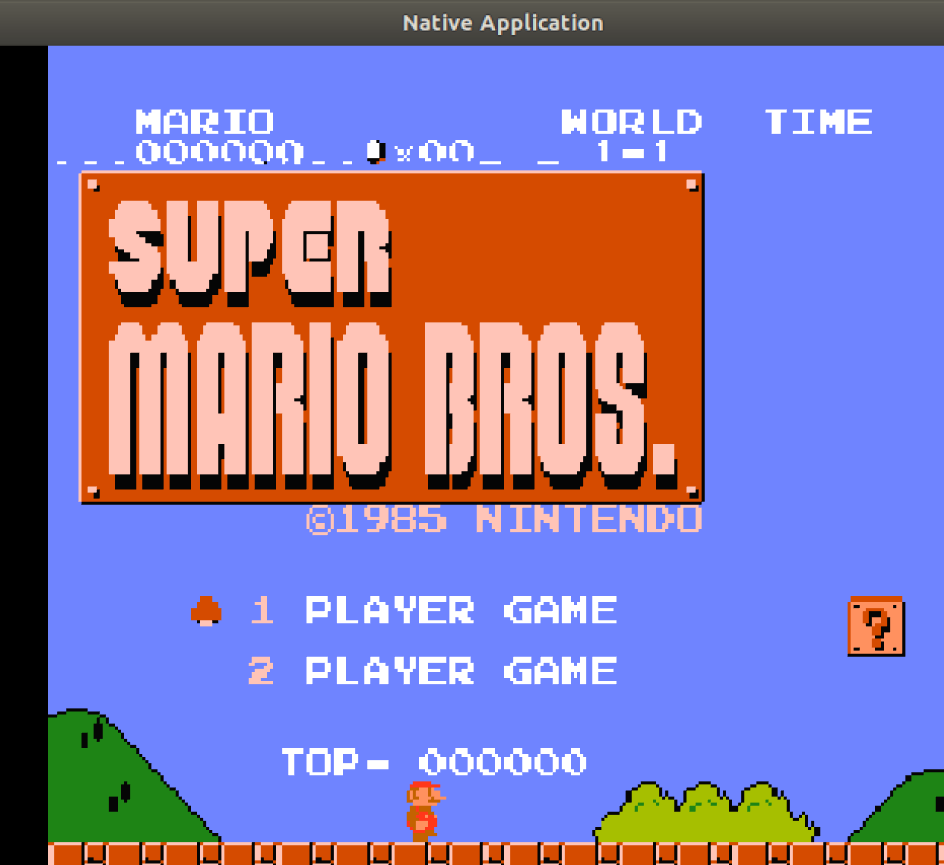
\includegraphics[scale=0.25]{fig/22.png}
        \caption{vga}
    \end{figure}
}
%---------------------------------------------------------------------------------------------------
\section{遇到的bug及解决}
\kt{
    收回PA1的话,PA1没有刁难,PA1进展太顺利了,PA2我重写了两次,不好好看指导书的锅orz
    \begin{itemize}
        \item 
        \begin{todolist}
            \item [\done] test指令的i386手册表述不是很明确,本意是不需要写与的结果的,这个STFW了一下才弄清除,只更新标志位就行了
            \item [\done] 有的RTL指令一定要记得用operand\_write到dest或者需要写的地方,标志位更新设置的顺序也一定要谨慎,再就是临时寄存器的使用一定要分清用在哪里,所以后来有一部分我直接赋给id\_dest了免得写着写着自己混乱了
            \item [\done] sar指令是需要借助SI还有msb等等进行符号扩展的毕竟是算术移位,否则会报错
            \item [\done] PA2教会了我:未测试的代码永远是错的,过了测试的代码也不一定是对的,暂且不提runall的All\ Combo,就光是从dummy到bit我的代码就撑不住了,而且尝试了各种方法都找不到原因,甚至还怀疑Machine有问题,还愚蠢的问到了老师面前,最后是重写了一遍(感谢分支技术和我备份的先见之明)靠着DiffTest找到了是前面shl还有sar的移位的标志位出了问题,靠着前面七零八落的Debug手段(Log)是真的完全找不出来
            \item [\done] 其实Copy-Paste是我以前经常干的事情,主要是真的很想偷懒,但是要注意的点太多了还不好debug所以这次,STFW几个printf的含义作用以及参考了不少代码,最终借助vsprintf避免了多与的Copy-Paste和Debug
            \item [\done] 外设的case的实现不声明需要的\#define也可以正常实现指导书要求的功能,但是回归测试的时候会报错,因为路径不一样了
            \item [\done] coremark跑分的时候有段错误,也是重新单个跑发现是imul的执行函数拼写问题
            \item [\done] 最早的几个测试样例就是哪里需要填指令就填哪里,这导致后面重复的指令还要重写exec.c,挺浪费时间的,所以从fib开始就一次性写完所有的指令,(虽然不用写完所有的也可以过测试就是了)
        \end{todolist}
    \end{itemize}
}
%---------------------------------------------------------------------------------------------------
\section{思考题\&\&必答题}
%——————————————————————————————————————
\subsection{思考题}
\kt{
    \begin{enumerate}
        \item 立即数背后的故事,假设我们需要将NEMU运行在Motorola 68k的机器上(把NEMU的源代码编译成Motorola 68k的机器码);假设我们需要编写一个新的模拟器NEMU-Motorola-68k, 模拟器本身运行在x86架构中, 但它模拟的是Motorola 68k程序的执行 
        
        情况一要注意的问题:内存中读取到的指令可能不会被正确的decode。原因:在大端机上,数据在内存中以大端方式存储,而NEMU是小端模式处理数据。解决方法:读内存之后对数据进行一定处理使数据符合小端模式的情景。
        
        情况二要注意的问题:同上。原因:x86机器中的数据在内存中是以小端方式存储的,NEMU-Motorola-68k是以大端方式处理数据的。解决方法:同上以保证NEMU-Motorola-68k仍可以使用自己的规则来对数据进行操作。
        \item 将运行时环境封装成库函数,现在不就只有NEMU这一个机器吗(m=1)? 哪里需要抽象?
        
        看ics2019就知道了,作者想到了多指令集所以就需要了,全都抽象成ISA的API调用,而在运行的时候指定ISA就可以了
        \item 堆和栈在哪里?
        
        为什么堆和栈的内容没有放入可执行文件里面?  
        
        auto类型的局部变量,他们在运行时被分配在栈中,所以他们既不在.data节中体现,也不在.bss节中出现。
        
        那程序运行时刻用到的堆和栈又是怎么来的? AM 的代码是否能给你带来一些启发?
        
        堆的创建是在程序运行时,用户栈总是从最大的合法用户地址开始(低地址方向),NEMU中的loader.ld文件\_stack\_pointer = 0x7c00;规定了栈的起始地址。在入口文件start.S中,调用mov指令将栈的开始位置传给寄存器esp。并在之后调用的\_trm\_init函数中,对堆的起始地址进行初始化。
        \item AT\&T格式反汇编结果中的少量指令, 与i386手册中列出的指令名称不符, 如cltd. 除了STFW之外, 你有办法在手册中找到对应的指令吗? 如果有的话, 为什么这个办法是有效的呢?
        
        先STFW这个指令的作用,在手册中查找有类似关键词的。比如cltd是Convert longword to doubleword的意思,翻手册的目录能找到意思差不多的Convert word to double word。或者看cltd的源码找到类似指令。
        \item 阅读相关Makefile和脚本文件, 尝试理解AM项目是如何生成native的可执行文件的.
        
        这一环套一环的Makefile看的人头晕,Makefile.compile里规定了native的编译参数,Makefile.lib里规定好路径还有lib文件,在terminal\ echo编译
        \item 为什么错误码是1呢? 你知道make程序是如何得到这个错误码的吗?
        
        string.c里面有nemu\_assert会使得程序中途出错的返回为false在makefile里面就会返回错误码1
        \item 作为一种基础设施, DiffTest能帮助你节省多少调试的时间呢?
        
        这个问题我好有发言权,就已经不是节省时间了,有的bug不用DiffTest比对甚至找不到根源,一点一点追根溯源的方法不仅不好找还浪费了好多时间,DiffTest的优点就是他可以最快找到对应错误的位置!
        \item 把思绪回归到PA中, 通用程序的性质告诉我们, NEMU的潜力是无穷的. 为了创造出一个缤纷多彩的世界, 你觉得NEMU还缺少些什么呢?
        
        缺少异常和中断,进程并行
        \item 你或许会感到疑惑, 代码优化不是一件好事情吗? 为什么会有volatile这种奇葩的存在? 思考一下, 如果代码中p指向的地址最终被映射到一个设备寄存器, 去掉volatile可能会带来什么问题?
        
        编译器是根据输入输出状态进行的代码优化,但作为人我们会考虑中间过程。如果代码中p指向的地址最终被映射到一个设备寄存器,可能会发生设备状态的跳变,比如显示器某块地方应该是由蓝变绿再变红,会直接从蓝色变成红色。
        \item 如何检测多个按键同时被按下?
        
        这个参考navy-apps/pps/litenes/src/fce.c里的fce\_run中判断按键部分,在外面再套一个while1死循环,当判断为——KEY\_NONE时跳出,否则就记录寄存器器状态,并反馈给用户。
    \end{enumerate}
}
%——————————————————————————————————————
\subsection{必答题}
\kt{
    必答题除了最后一部分,其余均为代码实现。
    \begin{enumerate}
        \item \underline{编译与链接} 在nemu/include/cpu/rtl.h中, 你会看到由static inline开头定义的各种RTL指令函数. 选择其中一个函数, 分别尝试去掉static, 去掉inline或去掉两者, 然后重新进行编译, 你可能会看到发生错误. 请分别解释为什么这些错误会发生/不发生? 你有办法证明你的想法吗?
        
        去掉static不会报错,去掉之后就是默认的extern声明,由于内存没有改变还是可以照样访问。

        去掉inline会报"defined but not used",inline是把函数里面的代码直接插入到调用这个函数的地方,而不是用调用函数的形式。如果函数体代码很短的话,会更有效率。但是inline是给编译器的提示,编译器会根据实际情况自己决定到底要不要进行内联,如果函数过大、有函数指针指向这个函数或者有递归的情况下编译器都不会进行内联。所以去掉inline之后,可能会因为没有引入该函数,而报其他地方调用失败的错误。

        都去掉会报"multiple definition of",inline相当于把一个函数固定在一个固定的内存里,即使没有static(不允许外部访问)但是由于内存没有改变所以还是能够访问。但是如果没有inline那就不能被外部访问了,如果都去掉,就会出现在两个内存中同时定义了这个函数,所以出现了重定义。
        \item \underline{编译与链接}
        \item \begin{enumerate}
            \item 在nemu/include/common.h中添加一行volatile static int dummy; 然后重新编译NEMU. 请问重新编译后的NEMU含有多少个dummy变量的实体? 你是如何得到这个结果的?
            
            应该是一个吧。。
            \item 添加上题中的代码后, 再在nemu/include/debug.h中添加一行volatile static int dummy; 然后重新编译NEMU. 请问此时的NEMU含有多少个dummy变量的实体? 与上题中dummy变量实体数目进行比较, 并解释本题的结果.
            
            两个,两个文件各一个,因为static只在当前文件起作用
            \item 修改添加的代码, 为两处dummy变量进行初始化:volatile static int dummy = 0; 然后重新编译NEMU. 你发现了什么问题? 为什么之前没有出现这样的问题? (回答完本题后可以删除添加的代码.)
            
            重定义报错,之前没有初始化且定义两个静态变量dummy,他们只在各自模块被引用,两个变量都有各自的分配空间,并作为两个不同的符号记录到符号表中,所以不会报错。但是初始化的值一样后就会报重定义的错。
        \end{enumerate}
        \item \underline{了解Makefile}
        
        读入Makefile,并且查看是否调用其他的Makefile;读取include文件的Makefile;初始化变量;为目标文件建立依赖关系;重新生成目标;执行
    \end{enumerate}
}
%----------------------------------------------------------------------------- 
\section{总结}
\kt{
    PA2一共多了264行代码,相比于PA1的394行少了些,大概原因是费时间的exec都不会增加新行吧.

    40h远远不止,时间跨度大约一个月吧,虽然中间空了20天因为bug什么也没干,但是还是很消耗脑力,代码能力重要,更重要的是找对方向,如果我早一点发现DiffTest的作用并且早一些时间,也许中间空闲的20天就不会束手无策了,AM那一章整体介绍都太长了,所以DiffTest就没有仔细看(非常后悔)。先看指导书,多看几遍看懂!然后再去RTFSC也许效果更好,太疲惫了,希望PA3能长点教训。

    另外,并没有实现PA1许下的快一点的诺言。希望下次不用快一点,别在bug上撞死就好。
}
%----------------------------------------------------------------------------- 
% \lhead{\kaishu 参考文献}
% \newpage
% \kt{
% \begin{thebibliography}{plain}  
%     \bibitem{ref1}Ray Tracing经典入门[EB/OL].https://raytracing.github.io/books/
%     \bibitem{ref2}讲稿lec2-5,8
% \end{thebibliography}
% }
\end{document}
